% !TeX root = ../main.tex
\chapter{Vehicle Stabilization}\label{chapter: stabilization}
Before start of the maneuvering step, vehicle should be set to the stabilized situation or that should be moved to a start position for maneuver. This step is also called positioning phase which is really important to make a collision free parking movement. Vehicle should have a correct starting position that is parallel to the front parked vehicle before entering to the parking place \cite{3phaseMobileRobot}. this step is considered as an interface between parking-detection(last chapter) and maneuvering step(chapter \ref{chapter:Parking Maneuver})
\begin{figure}
    \centering
    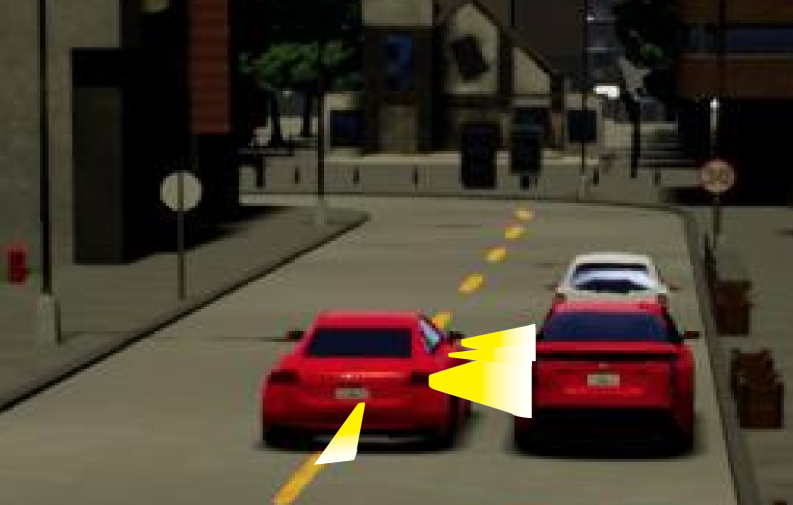
\includegraphics[width=7cm, height=5cm]{images/sensorPlace.png}
    \caption{Sensor places in ego-vehicle}
    \label{fig:sensorPlaces}
\end{figure}
\ref{chapter:Parking Maneuver}.
After the estimation of parking vacancy, vehicle moves slowly to the parking place and during this movement, sensors in the right side of the car are started. Sensors provide information of non-player vehicles' location cover the empty parking space(parking vacancy). Based on the exact distance between two non-player cars, L(length of the parking place) and W(width of the parking) could be measured. values of L and W are used in the next step to make parking maneuver algorithm. When the vehicle reach to the second non-player vehicle(after passing empty space), it should be stopped and prepared for parking. In this work there are three sensors in the right side of the vehicle. Fig \ref{fig:sensorPlaces} illustrates place of the sensors. Each of the sensors give the distance to the detected-vehicle. When ego reaches to the location of second car(after passing parking space), distance between ego-vehicle and this car is measured by three sensors. If all sensors show the same distance value, it means that ego-vehicle is parallel to the non-player car and should be stopped at this point. Fig \ref{fig:startPosition}) shows the starting position of the vehicle before moving to the parking lot.
\begin{figure}
    \begin{tabular}{c|c}
         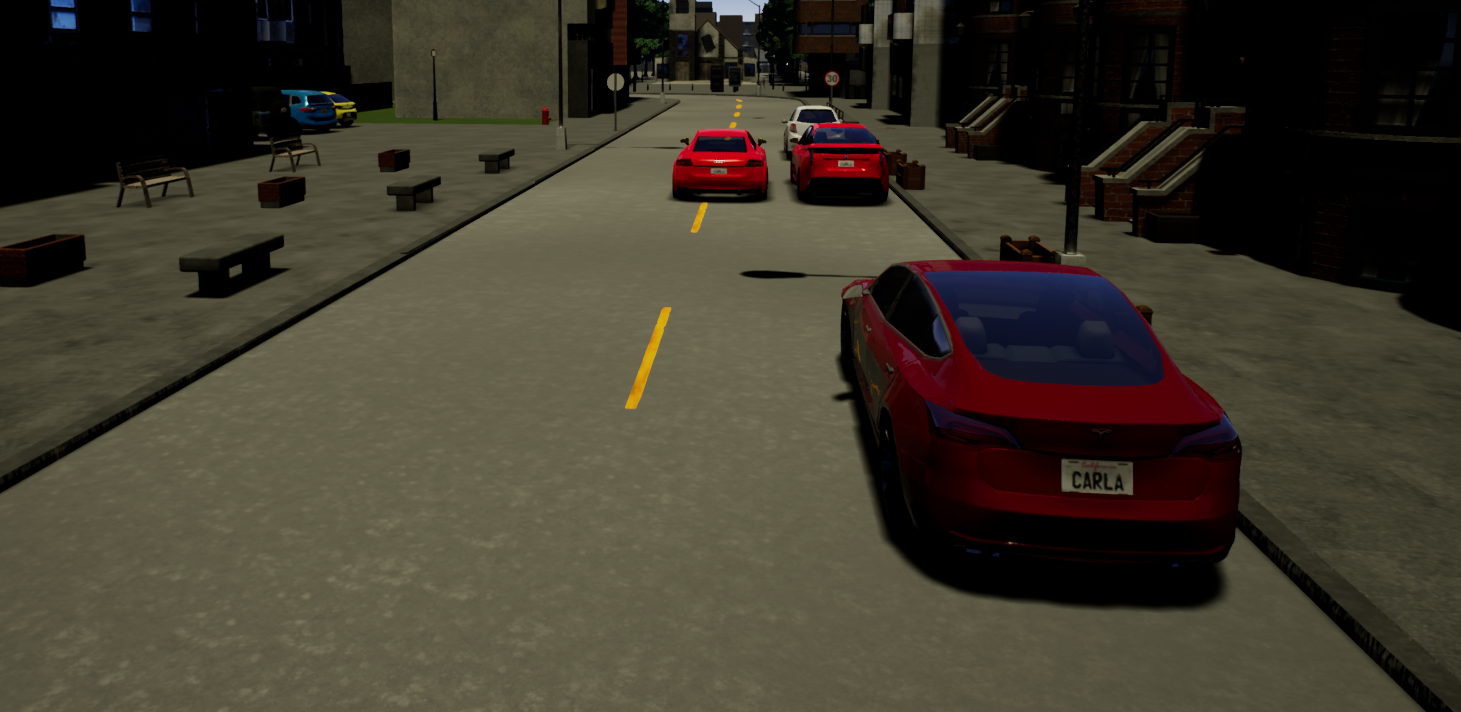
\includegraphics[width=7cm, height=4cm]{images/position1.png} 
         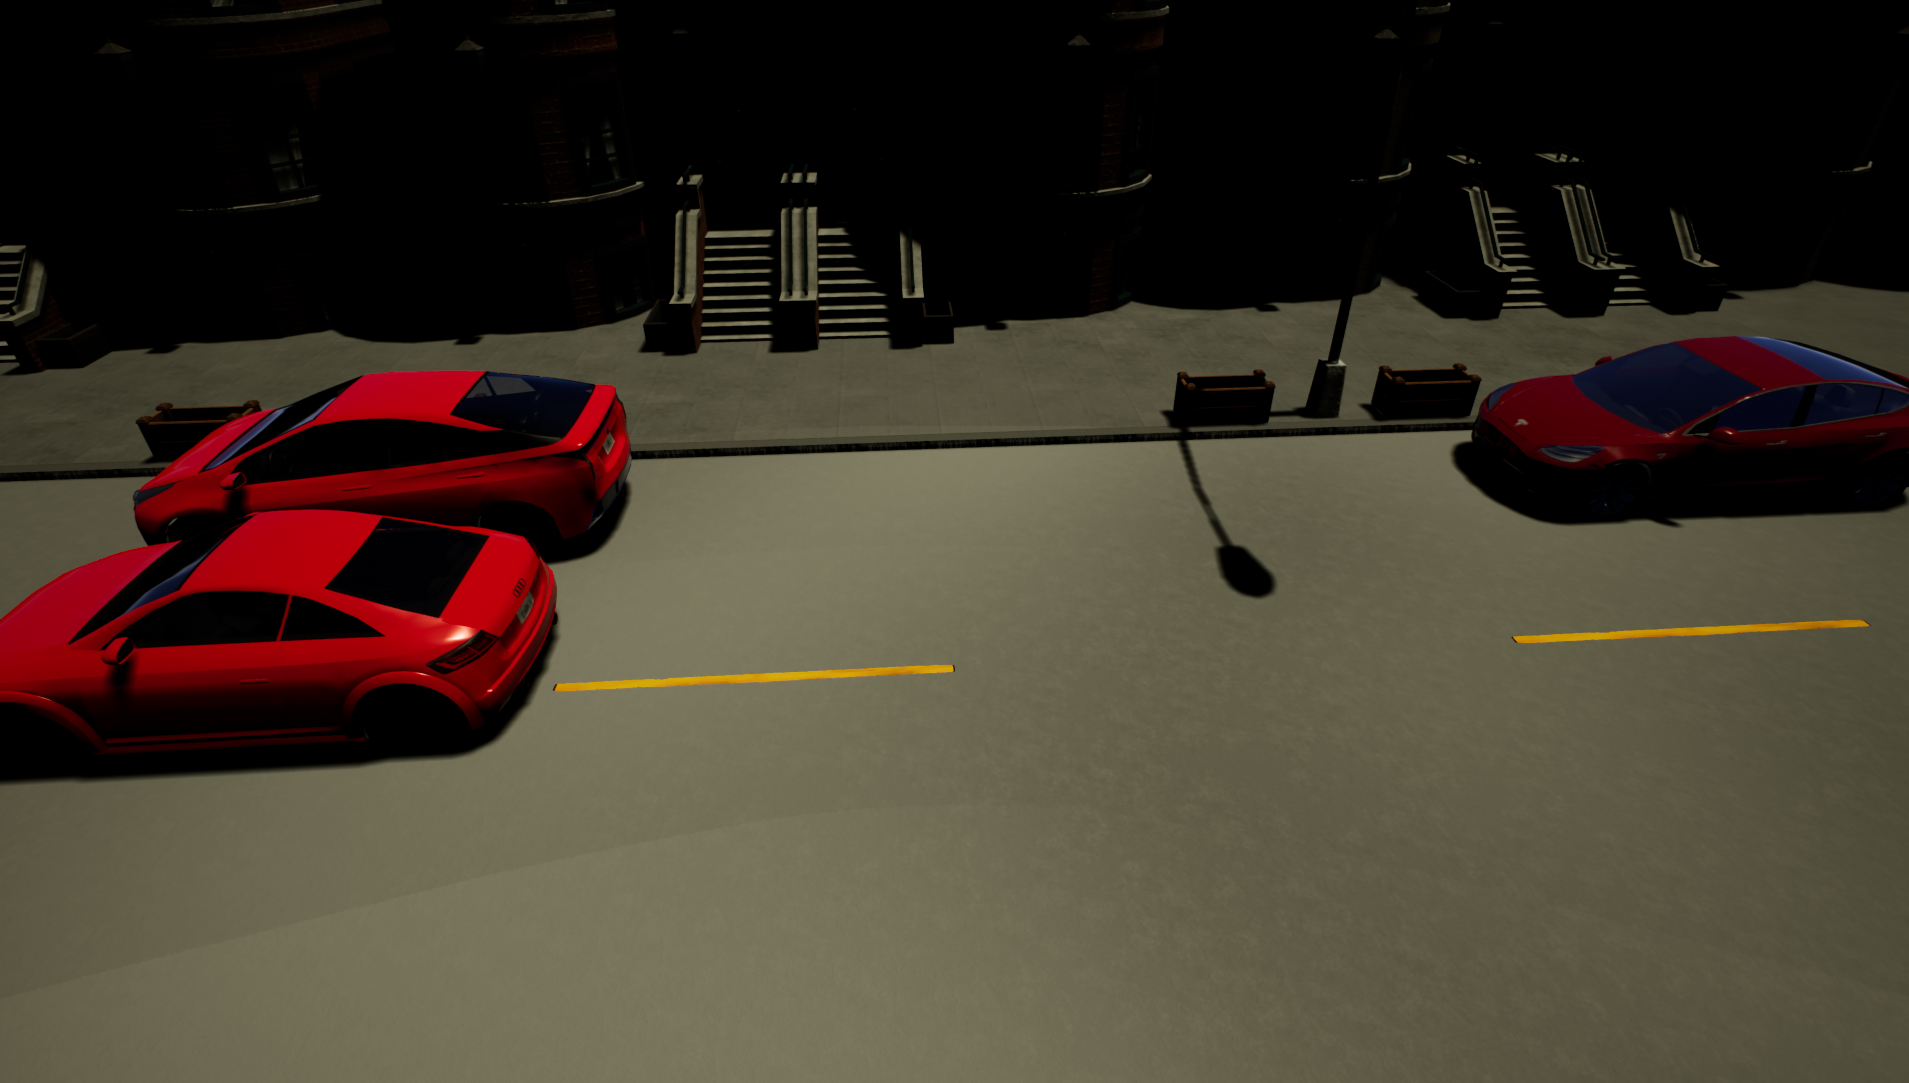
\includegraphics[width=7cm, height=4cm]{images/position2.png}
    \end{tabular}
    \caption{Start of Parking Maneuver}
    \label{fig:startPosition}
\end{figure}

